\documentclass[a4paper, 10pt]{article}

\usepackage{vmargin}

\setmarginsrb{2cm}{0cm}{2cm}{0,2cm}{1cm}{1,5cm}{1cm}{1,5cm}
%1 est la marge gauche
%2 est la marge en haut
%3 est la marge droite
%4 est la marge en bas
%5 fixe la hauteur de l'entête
%6 fixe la distance entre l'entête et le texte
%7 fixe la hauteur du pied de page
%8 fixe la distance entre le texte et le pied de page
%------------------------------Packages généraux------------------------------

\usepackage[english]{babel}
\usepackage[T1]{fontenc}
\usepackage{ae}
\usepackage[utf8]{inputenc}
\usepackage{scrextend}
\usepackage{hyperref}

%-------------------------Mathématiques------------------------------
\usepackage{amsmath}
\usepackage{amssymb}
\usepackage{amsthm}
\usepackage{amsfonts}
\usepackage{eucal}
\newcommand\independent{\protect\mathpalette{\protect\independenT}{\perp}}
\def\independenT#1#2{\mathrel{\rlap{$#1#2$}\mkern2mu{#1#2}}}
%-----------------------Codes et algorithmes--------------------------
\usepackage{algorithm}
\usepackage{algorithmic}
\usepackage{clrscode3e}

%------------------------------Graphics------------------------------

\usepackage{graphicx}
\usepackage{fancyhdr}
\usepackage{fancybox}
\usepackage{color}
\usepackage{pgf, tikz}
\usetikzlibrary{arrows, automata}
%\usepackage{slashbox}
%------------------------------Syntaxe------------------------------

\usepackage{listings}
\lstloadlanguages{Matlab}

\def\refmark#1{\hbox{$^{\ref{#1}}$}}
\DeclareSymbolFont{cmmathcal}{OMS}{cmsy}{m}{n} %Mathcal correcte
\DeclareSymbolFontAlphabet{\mathcal}{cmmathcal}

%------------------------------Inclure code MatLab------------------------------

\usepackage{listings}
\newcommand*\styleC{\fontsize{9}{10pt}\usefont{T1}{ptm}{m}{n}\selectfont }
\newcommand*\styleD{\fontsize{9}{10pt}\usefont{OT1}{pag}{m}{n}\selectfont }

%------------------Sub-sections--------%
\usepackage{titlesec}
\usepackage{hyperref}

\renewcommand\thesubsubsection{\alph{subsubsection}}

\titleclass{\subsubsubsection}{straight}[\subsubsection]

\newcounter{subsubsubsection}[subsubsection]
\renewcommand\thesubsubsubsection{\thesubsubsection.\arabic{subsubsubsection}}

\titleformat{\subsubsubsection}
  {\normalfont\normalsize\bfseries}{\thesubsubsubsection}{1em}{}
\titlespacing*{\subsubsubsection}
{0pt}{3.25ex plus 1ex minus .2ex}{1.5ex plus .2ex}


\makeatletter
% on fixe le langage utilisé
\lstset{language=matlab}
\edef\Motscle{emph={\lst@keywords}}
\expandafter\lstset\expandafter{%
  \Motscle}
\makeatother


\definecolor{Ggris}{rgb}{0.45,0.48,0.45}

\lstset{emphstyle=\rmfamily\color{blue}, % les mots réservés de matlab en bleu
basicstyle=\styleC,
keywordstyle=\ttfamily,
commentstyle=\color{Ggris}\styleD, % commentaire en gris
numberstyle=\tiny\color{red},
numbers=left,
numbersep=10pt,
lineskip=0.7pt,
showstringspaces=false}
%  % inclure le fichier source
\newcommand{\FSource}[1]{%
\lstinputlisting[texcl=true]{#1}
}

\usepackage[section]{placeins}

\let\cleardoublepage\clearpage

\usepackage{hyperref}
               
 \hypersetup{
    colorlinks = true,
    linkcolor=black,
    urlcolor = black
    }
%------------------------------Début du document------------------------------
\begin{document}
%------------------------------Page de garde------------------------------


  % \frontmatter
  %\tableofcontents
   \setcounter{page}{1}
   %%%%%%%%% TP 4 %%%%%%%%%%%
   \section{Representing uncertain knowledge (08/11/2018)}
   \subsection{Objectives}
      At the end of this repetition you should be able to:
      \begin{itemize}
          \item Apply Bayes rules, independence and marginalisation appropriately to compute probabilities
          \item Define, construct a Bayesian network
          \item Compute probabilities in the context of a simple Bayesian network.
      \end{itemize}
\subsection{Exercises}
   \subsubsection{$\approx 10$ min}
   Let two events A, B of the probability space $\Omega$; Is it possible to get $P(A)=0.4$, $P(B)=0.3$, and
    $P(A\vee B)=0.5$? If so, what range of probabilities would be possible for $A\wedge B$?
    \subsubsection{$\approx 15$ min}
    Given the probability table of Figure \ref{fig:p_table} compute the following probabilities:
    \begin{enumerate}
        \item P(toothache)
        \item P(cavity)
        \item P(toothache | cavity)
        \item P(cavity | toothache $\vee$ catch)
    \end{enumerate}
    \begin{figure}[H]
        \centering
        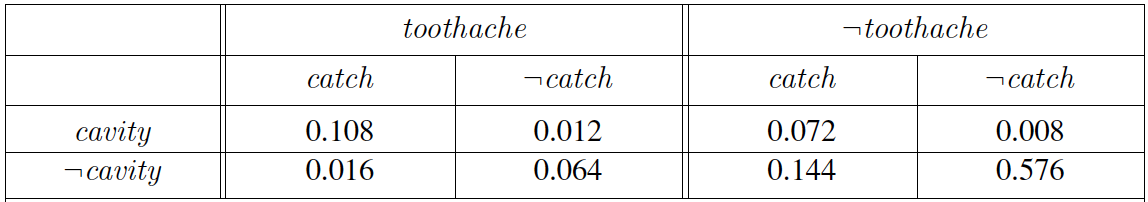
\includegraphics[width=1.\textwidth]{figures/proba_table.png}
        \caption{Probablity Table of Toothache and Cavity}
        \label{fig:p_table}
    \end{figure}
    \subsubsection{$\approx 10$ min}
    After your yearly checkup, the doctor has bad news and good news. The bad news
is that you tested positive for a serious disease and that the test is 99\% accurate (i.e., the
probability of testing positive when you do have the disease is 0.99, as is the probability of
testing negative when you don’t have the disease). The good news is that this is a rare disease,
striking only 1 in 10,000 people of your age. Why is it good news that the disease is rare?
What are the chances that you actually have the disease?
\subsubsection{$\approx 20$ min}
We have a bag of three biased coins a, b, and c with probabilities of coming up heads
of 20\%, 60\%, and 80\%, respectively. One coin is drawn randomly from the bag (with equal
likelihood of drawing each of the three coins), and then the coin is flipped three times to
generate the outcomes X1, X2, and X3.
\begin{enumerate}
    \item Draw the Bayesian network corresponding to this setup and define the necessary CPTs.
    \item Calculate which coin was most likely to have been drawn from the bag if the observed
flips come out heads twice and tails once.
\end{enumerate}
\subsubsection{$\approx 30$ min}
Let $H_x$ be a random variable denoting the handedness of an individual $x$, with possible
values $l$ or $r$. A common hypothesis is that left- or right-handedness is inherited by a simple
mechanism; that is, perhaps there is a gene $G_x$, also with values l or r, and perhaps actual
handedness turns out mostly the same (with some probability s) as the gene an individual
possesses. Furthermore, perhaps the gene itself is equally likely to be inherited from either
of an individual’s parents, with a small nonzero probability m of a random mutation flipping
the handedness.
\begin{enumerate}
    \item Which of the three networks in Figure \ref{fig:b_net} claim that\\ $P(G_{father},G_{mother},G_{child}) =
P(G_{father} )P(G_{mother} )P(G_{child} )$?
    \item Which of the three networks make independence claims that are consistent with the
    \item Which of the three networks is the best description of the hypothesis?
    \item Write down the CPT for the Gchild node in network (a), in terms of s and m.
    \item Suppose that $P(G_{father} =l) = P(G_{mother} =l) = q$. In network (a), derive an expression
for $P(G_{child} =l)$ in terms of m and q only, by conditioning on its parent nodes.
    \item Under conditions of genetic equilibrium, we expect the distribution of genes to be the
same across generations. Use this to calculate the value of q, and, given what you know
about handedness in humans, explain why the hypothesis described at the beginning of
this question must be wrong.
hypothesis about the inheritance of handedness?
\end{enumerate}
\begin{figure}[H]
    \centering
    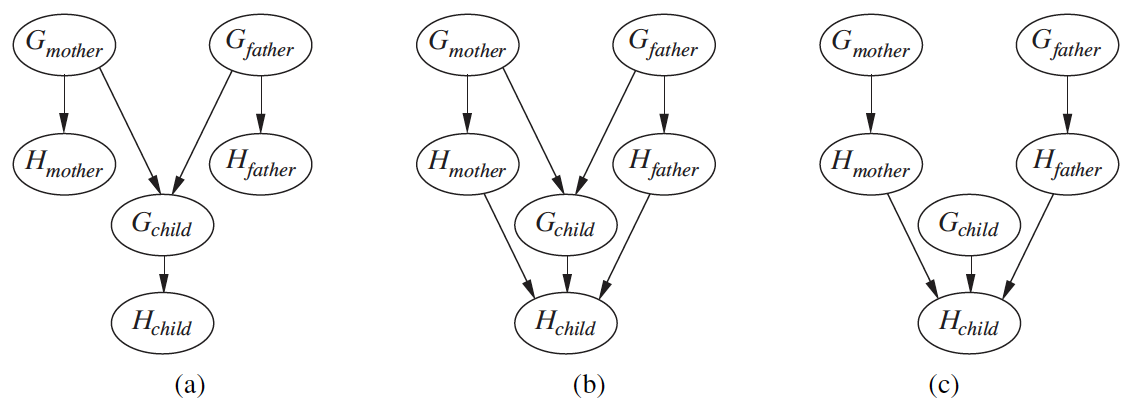
\includegraphics[width=1.\textwidth]{figures/bnet.png}
    \caption{Possible Bayesian Networks of handedness inheritance}
    \label{fig:b_net}
\end{figure}
\subsubsection{$\approx 5$ min}
\begin{figure}[H]
    \centering
    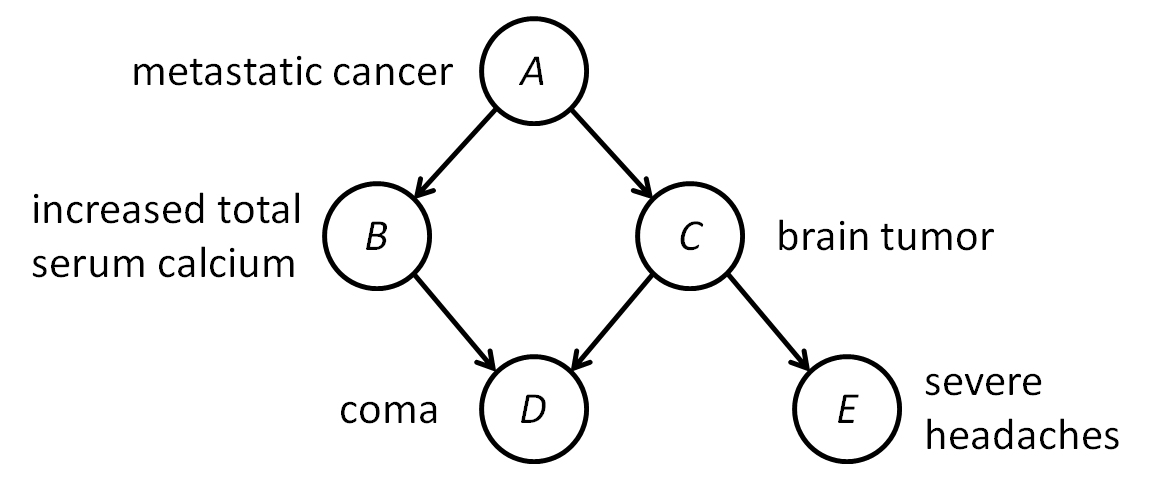
\includegraphics[width=1.\textwidth]{figures/pearl-bn-example.png}
    \caption{Bayesian Network of metastatic cancer}
    \label{fig:pearl-b-net}
\end{figure}
Consider the Bayesian network of Figure \ref{fig:pearl-b-net}, which, if any, of the following are asserted by the network structure?
\begin{itemize}
    \item $P(B, C) = P(B)P(C)$
    \item $P(B, C|A) = P(B|A)P(C|A)$
    \item $P(B, C| A, D) = P(B|A, D) P(C|A, D)$
    \item $P(C|A, D, E) = P(C|A, B, D, E)$
    \item $P(B, E) = \sum_{A, C, D} P(A) P(B|A) P(C|A) P(E|C) P(D|B, C)$
\end{itemize}

   \subsection{Supplementary material}
   \url{https://www.youtube.com/watch?v=x-2uVNze56s}
   
 
   
   
\end{document}
